\chapter{Gaokao Reform --- Equal Probability Admission}\label{app:gaokao}

The preceding appendix applied the framework to the fiscal substrate
of sovereign debt (\cref{app:govfi}).  This appendix applies it to
the \emph{human capital substrate}---the university admission system
that determines which agents enter the viability kernel of higher
education.  The central result is a \emph{disparity conservation law}:
total university capacity is conserved; only its distribution across
provinces is free.  The policy implication is that the current allocation
system is a \emph{knife}---a structural separator that assigns students
different viability probabilities based solely on their province of
registration---and that a population-proportional allocation
removes this knife entirely.

% ================================================================
\paragraph{Notation / 符号表.}
% ================================================================
The following symbols are used throughout this appendix.
\textcolor{water}{Blue} = structure/flow,
\textcolor{knife}{red} = disparity/inequality,
\textcolor{sword}{cyan} = reform/detection,
\textcolor{caution}{orange} = threshold warnings.

\begin{center}
\renewcommand{\arraystretch}{1.2}
\begin{tabular}{@{}lp{5.5cm}p{5.5cm}@{}}
\toprule
\textbf{Symbol} & \textbf{English} & \textbf{中文} \\
\midrule
\multicolumn{3}{@{}l}{\emph{Provincial state}} \\
$N_i$             & Exam takers in province $i$
                  & 第 $i$ 省报名人数 \\
$n$               & Number of provinces ($= 31$)
                  & 省份数 \\
$C$               & Total national 985 capacity
                  & 985 总招生容量 \\
$s_i$             & Slots allocated to province $i$
                  & 第 $i$ 省招生名额 \\
\midrule
\multicolumn{3}{@{}l}{\emph{Rates / 录取率}} \\
$R_i$             & Admission rate $= s_i / N_i$
                  & 录取率 \\
$\bar{R}$         & National avg $= C / \sum N_i$
                  & 全国平均录取率 \\
\midrule
\multicolumn{3}{@{}l}{\emph{Disparity / 不平等}} \\
$D$               & Disparity ratio $= \max R_i / \min R_i$
                  & 最大最小比 \\
$G$               & Gini coefficient of $\{R_i\}$
                  & 基尼系数 \\
$\sigma_R$        & Std.\ dev.\ of rates across provinces
                  & 录取率标准差 \\
\midrule
\multicolumn{3}{@{}l}{\emph{Reform models}} \\
$w_i$             & Province weight (equal: $w_i = 1$)
                  & 省份权重 \\
$\Delta$          & Score band width (points)
                  & 分数段宽度 \\
\bottomrule
\end{tabular}
\end{center}

% ================================================================
\section{The Current System / 现行制度}\label{sec:gaokao-current}
% ================================================================

China's national college entrance examination (高考) is taken by
approximately $N = \sum_{i=1}^{31} N_i \approx 12{,}350{,}000$
students annually (2024 data).  Each university allocates a
\emph{fixed quota} $s_i$ to each province, set by historical
precedent and political negotiation rather than by population
proportion.  The admission rate for province~$i$ is
\begin{equation}\label{eq:gaokao-rate}
  R_i = \frac{s_i}{N_i}.
\end{equation}

\begin{definition}[Disparity index / 不平等指数]\label{def:disparity}
The \emph{disparity ratio} is $D = \max_i R_i \;/\; \min_i R_i$.
The \emph{Gini coefficient} of the rate vector $\mathbf{R}
= (R_1, \ldots, R_n)$ is
\[
  G = \frac{1}{2n^2 \tilde{R}} \sum_{i,j} |R_i - R_j|,
  \qquad \tilde{R} = \frac{1}{n}\sum_i R_i.
\]
Perfect equality: $G = 0$, $D = 1$.
Maximum inequality: $G \to 1$, $D \to \infty$.
\end{definition}

\paragraph{2024 data / 2024年数据.}
Using publicly available data from Chinese education statistics
sources\footnote{%
  Sources: 中国教育在线 (eol.cn), 聚汇数据 (gotohui.com),
  知乎 (zhihu.com), 高考直通车 (gaokaozhitongche.com),
  网易 (163.com), 搜狐 (sohu.com).
  All figures are approximate; see \texttt{gaokao/data.py} for
  per-source annotations and confidence levels.},
the 2024 985-university admission rates are:

\begin{center}
\renewcommand{\arraystretch}{1.1}
\begin{tabular}{@{}llrr@{}}
\toprule
\textbf{Province / 省份} & & \textbf{Exam takers / 考生}
  & \textbf{985 rate / 录取率} \\
\midrule
\multicolumn{4}{@{}l}{\emph{Top 5 — highest rate / 录取率最高}} \\
天津 & Tianjin   &   70{,}800 & 5.81\% \\
北京 & Beijing   &   67{,}000 & 5.30\% \\
上海 & Shanghai  &   54{,}000 & 4.40\% \\
吉林 & Jilin     &  130{,}100 & 3.56\% \\
青海 & Qinghai   &   65{,}600 & 3.36\% \\
\midrule
\multicolumn{4}{@{}l}{\emph{Bottom 5 — lowest rate / 录取率最低}} \\
云南 & Yunnan    &  395{,}000 & 1.00\% \\
广东 & Guangdong &  768{,}000 & 0.98\% \\
贵州 & Guizhou   &  472{,}500 & 0.98\% \\
河北 & Hebei     &  928{,}000 & 0.96\% \\
河南 & Henan     & 1{,}360{,}000 & 0.84\% \\
\bottomrule
\end{tabular}
\end{center}

\begin{proposition}[2024 disparity / 2024年不平等]\label{prop:gaokao-disparity}
For 985-university admission rates across 31 provinces (2024):
\[
  D = 6.9\times, \qquad G = 0.310, \qquad
  \bar{R}_{\textup{weighted}} = 1.33\%.
\]
天津 (Tianjin, $N = 70{,}800$) has a 985 rate of $5.81\%$;
河南 (Henan, $N = 1{,}360{,}000$) has $0.84\%$.
河南 has $19\times$ more exam takers but $6.9\times$ worse
admission probability.
\end{proposition}

\begin{remark}[The knife is the quota / 刀就是名额]
\label{rem:gaokao-knife}
The admission quota $s_i$ is the knife.  It satisfies both conditions
from \cref{def:knife}: (1)~autonomous actuation---each university
sets its own quotas without external constraint; (2)~observability
failure---students in province $i$ cannot observe or influence the
quota-setting process.  The disparity $D = 6.9\times$ is not a
natural phenomenon; it is an artefact of the quota allocation,
which is neither population-proportional nor merit-based.
\end{remark}

% ================================================================
\section{Reform Models / 改革模型}\label{sec:gaokao-reform}
% ================================================================

We consider two alternative allocation rules, holding total
capacity $C = \sum_i s_i \approx 164{,}203$ fixed.

\begin{definition}[Equal-weight allocation / 等权分配]
\label{def:equal-weight}
Set $w_i = 1$ for all $i$.  Then
\[
  s_i^{\textup{eq}} = \frac{C}{n}
  \approx 5{,}297 \;\text{per province}.
\]
\end{definition}

\begin{definition}[Population-proportional allocation / 人口比例分配]
\label{def:pop-prop}
Set $w_i = N_i$.  Then
\[
  s_i^{\textup{pp}} = C \cdot \frac{N_i}{\sum_j N_j},
  \qquad
  R_i^{\textup{pp}} = \frac{s_i^{\textup{pp}}}{N_i}
  = \frac{C}{\sum_j N_j} = \bar{R}
  \;\;\text{(constant for all $i$)}.
\]
\end{definition}

\begin{proposition}[Reform comparison / 改革对比]
\label{prop:gaokao-reform}
Under the three allocation models:
\begin{center}
\renewcommand{\arraystretch}{1.1}
\begin{tabular}{@{}lrrr@{}}
\toprule
\textbf{Model / 模型} & \textbf{Gini ($G$)} & \textbf{$D$ (max/min)}
  & \textbf{Direction} \\
\midrule
Current / 现行制度  & $0.310$ & $6.9\times$ & --- \\
Equal-weight / 等权 & $0.514$ & $37.8\times$
  & \textcolor{knife}{$\uparrow$ worse} \\
Pop-proportional / 人口比例 & $0.0001$ & $1.0\times$
  & \textcolor{sword}{$\downarrow$ optimal} \\
\bottomrule
\end{tabular}
\end{center}
\end{proposition}

\begin{remark}[等权 $\neq$ 等概率 / Equal weight $\neq$ equal probability]
\label{rem:eq-neq-eqprob}
The na\"ive intuition that ``equal provincial weight'' produces
equality is \textbf{wrong}.  Equal absolute slots ($C/n$) distributed
to provinces of vastly different population sizes produces
\emph{worse} per-capita disparity: 西藏 ($N = 36{,}000$) would receive
a $14.7\%$ rate while 河南 ($N = 1{,}360{,}000$) would receive $0.39\%$.
The disparity ratio rises from $6.9\times$ to $37.8\times$.

The correct reform is population-proportional allocation:
$s_i \propto N_i$.  This gives every student the same probability
$R_i = \bar{R} \approx 1.33\%$ regardless of province.
\end{remark}

\begin{theorem}[Proportional allocation eliminates the knife]
\label{thm:gaokao-knife-removal}
Under population-proportional allocation $s_i = C \cdot N_i / N$
where $N = \sum_j N_j$:
\begin{enumerate}[label=\textup{(\alph*)}]
\item $R_i = C/N = \bar{R}$ for all $i$ (uniform rate);
\item $G = 0$ and $D = 1$ (perfect equality);
\item The quota $s_i$ ceases to be a knife: it no longer separates
  viability classes by province.
\end{enumerate}
\end{theorem}

\begin{proof}
(a) is immediate from the definition.  (b) follows since all rates are
equal.  For~(c), the knife conditions (\cref{def:knife}) fail:
the allocation is now a deterministic function of the publicly
observable population $N_i$, so observability holds and no autonomous
actuation remains.
\end{proof}

% ================================================================
\section{Within-Band Randomization / 分数段内随机化}
\label{sec:gaokao-band}
% ================================================================

The current system ranks students by exact score within each province.
A difference of one point (满分750, so $\Delta s = 1/750 \approx 0.13\%$
of the total range) can determine admission or rejection.  This creates
a ``one-point-one-fate'' (一分定终身) phenomenon.

\begin{definition}[Band randomization / 分数段随机化]
\label{def:band-random}
Fix a band width $\Delta > 0$ (e.g., $\Delta = 5$ points).
Partition the score range $[0, 750]$ into bands
$B_k = [k\Delta, (k+1)\Delta)$.
Within each band $B_k$, students are ranked by
\emph{uniform random permutation} rather than exact score.
\end{definition}

The effect: students whose scores differ by less than $\Delta$ have
equal probability of admission.  This converts a deterministic
(and fragile) ranking into a probabilistic one, eliminating the
incentive for one-point gaming while preserving the overall
meritocratic ordering at the $\Delta$-scale.

\begin{remark}[Band width choice / 分数段宽度选择]
\label{rem:band-width}
The choice $\Delta = 5$ is illustrative.  The optimal $\Delta$
balances two competing effects:
\begin{itemize}
\item Too small ($\Delta = 1$): equivalent to exact ranking,
  no randomization benefit.
\item Too large ($\Delta = 50$): too much noise, weakens
  the meritocratic signal.
\end{itemize}
The right $\Delta$ is an empirical question requiring the
fine-grained score distribution (一分一段表) to calibrate.
Score distributions for 2024 are publicly available for 29 of 31
provinces from provincial education examination authorities.
\end{remark}

% ================================================================
\section{Grace Period / 恩典期}\label{sec:gaokao-grace}
% ================================================================

The within-band randomization (\cref{sec:gaokao-band}) assigns each
student a \emph{tentative} school placement.  This initial assignment
is random within the score band.  The grace period converts this
random assignment into a \emph{chosen} one.

\begin{definition}[Grace period / 恩典期]\label{def:grace-period}
After the initial random-within-band assignment, a grace window
$[t_0, t_0 + \tau]$ opens during which students may \emph{swap}
placements with any other student in the same score band and the
same region, subject to the constraint that both students remain
within the same admission tier (budget).
\end{definition}

The mechanism has three phases:
\begin{enumerate}[label=\textup{(\alph*)}]
\item \textbf{Random seed / 随机初始.}
  Within-band randomization produces an initial assignment.
  No student chose this placement; it is the system's first offer.
\item \textbf{Grace window / 恩典窗口.}
  Students examine their assignment and may swap with willing
  partners in the same band and region.  You keep your tier
  but choose your specific school.  This is the time for the
  考生 to think: where do I actually want to go?
\item \textbf{Lock / 锁定.}
  After $\tau$, assignments become final.  No further swaps.
\end{enumerate}

\begin{remark}[Grace as bounded dissipation / 恩典即有界耗散]
\label{rem:gaokao-grace}
This is the same structure as the GovFi grace margins
(\cref{app:govfi}): bounded freedom within thresholds.
In GovFi, each layer $i$ has a grace margin $\epsilon_i = k_i - r$
within which losses are tolerated as legitimate costs.
In Gaokao, each student has a grace margin: freedom to swap
within the same tier without affecting the system's aggregate
allocation.

The grace period restores agency without restoring the knife.
The initial randomization removes one-point-one-fate (一分定终身);
the grace period gives back the student's choice of \emph{where},
while the population-proportional allocation determines \emph{how many}.
The constraint is the tier, not the specific school.

What is consumed during the grace period---the dissipated---is
information: students learn about their options, negotiate swaps,
discover preferences.  This is bounded dissipation in information
space, exactly analogous to the fiscal grace in \cref{app:govfi}.
\end{remark}

% ================================================================
\section{The Mean-Field Connection / 平均场联系}
\label{sec:gaokao-meanfield}
% ================================================================

The Gaokao disparity is a mean-field phenomenon in the sense of
\cref{sec:meanfield}.

\begin{proposition}[Knife = quota, mean = population share]
\label{prop:gaokao-meanfield}
Let $\bar{R} = C/N$ be the population-weighted national average.
Then:
\begin{enumerate}[label=\textup{(\alph*)}]
\item $13$ provinces (containing $67\%$ of all exam takers)
  have $R_i < \bar{R}$.
\item $18$ provinces (containing $33\%$ of all exam takers)
  have $R_i \geq \bar{R}$.
\item The unweighted arithmetic mean
  $\tilde{R} = \frac{1}{n}\sum R_i = 1.94\%$ exceeds $\bar{R} = 1.33\%$,
  showing that \emph{the majority of provinces have above-average rates
  when measured per province, but the majority of students have
  below-average rates when measured per capita}.
\end{enumerate}
\end{proposition}

This is the knife-is-the-mean phenomenon: the average computed
per province (unweighted, $\tilde{R}$) differs from the average
computed per student (weighted, $\bar{R}$), and this discrepancy
is itself the knife.  Most provinces appear ``above average'' while
most students are below it.

\begin{remark}[Importance sampling / 重要性抽样]
\label{rem:importance-sampling}
Why do the two averages disagree?  Because the current system
assigns importance weights in two levels:
\begin{enumerate}[label=\textup{(\arabic*)}]
\item \textbf{Level 1: equally to each province.}
  Every province gets the same voice---Tibet (3.6 万考生)
  counts the same as Henan (136 万考生), a 38:1 population
  ratio compressed to 1:1.
\item \textbf{Level 2: equally to each student within that province.}
  Within each province, students share their province's voice
  equally.
\end{enumerate}
The result: a student in Tibet inherits $1/36{,}000$ of a
full provincial vote, while a student in Henan inherits
$1/1{,}360{,}000$ of the same-sized vote.  Tibet's student
is 38 times louder than Henan's.  The importance weights
are the seed you plant---and the current system plants
unequal seeds.

In statistics, the fix is called \textbf{importance sampling}
(重要性抽样): if your sampling distribution $q$ differs from
the true distribution $p$, you multiply each sample by a
\emph{correction weight} $w(x) = p(x)/q(x)$:
\[
  \mathbb{E}_p[f(x)]
  \;=\;
  \mathbb{E}_q\!\Bigl[f(x)\,\cdot\,\frac{p(x)}{q(x)}\Bigr].
\]
Here $p$ is the per-student distribution (province $i$ has weight
$N_i/N$), $q$ is the per-province distribution (each province has
weight $1/n$), and $f$ is the admission rate.  The importance
weight is:
\[
  w_i \;=\; \frac{p_i}{q_i}
  \;=\; \frac{N_i/N}{1/n}
  \;=\; \frac{n\,N_i}{N}.
\]
Large provinces get large weights (Henan: $w \approx 3.4$),
small provinces get small ones (Tibet: $w \approx 0.09$).
The weighted average $\bar{R} = \sum w_i R_i / \sum w_i = 1.33\%$
is the true per-student mean.  The unweighted average
$\tilde{R} = 1.94\%$ is the \emph{biased} estimate that
ignores population---it over-counts small privileged provinces
and under-counts large disadvantaged ones.

In plain language (大白话): the unweighted mean is biased because
it lets 3.6 万 people in Tibet speak as loudly as 136 万 in Henan.
Importance sampling says: if you insist on giving every province
one vote, at least \emph{weight} those votes by how many students
each province actually has.  Once you do, $\tilde{R}$ collapses
to $\bar{R}$, and the illusion that ``most provinces are above
average'' disappears.
\end{remark}

\begin{remark}[Renormalization / 重整化]
\label{rem:gaokao-rg}
The importance weight assignment is a
\textcolor{knife}{renormalization group (RG) flow} compressed
into a single exam paper.  The current system has two scales:
\begin{center}
\renewcommand{\arraystretch}{1.15}
\begin{tabular}{@{}lll@{}}
\toprule
Scale & \textcolor{knife}{Current (bare)} & \textcolor{sword}{Reform (fixed point)} \\
\midrule
\textbf{Province} (coarse) & weight $= 1/n$ each
  & weight $= N_i/N$ \\
\textbf{Student} (fine) & weight $= 1/(n N_i)$
  & weight $= 1/N$ \\
\bottomrule
\end{tabular}
\end{center}
Under the \textcolor{knife}{current system}, the per-student
weight \emph{runs} with the province size $N_i$: a Tibet student
carries weight $1/(31 \times 36{,}000)$ while a Henan student
carries $1/(31 \times 1{,}360{,}000)$---a factor of 38.
The ``coupling constant'' (per-student admission probability)
\textcolor{knife}{depends on the scale at which you observe it}.
This is the signature of a system away from its RG fixed point.

Under \textcolor{sword}{population-proportional allocation}, every
student carries weight $1/N$ regardless of province.
The coarse-grained answer (per province: $s_i/N_i = C/N$)
and the fine-grained answer (per student: $C/N$) \emph{agree}.
The coupling no longer runs.
\textcolor{sword}{This is the RG fixed point}:
the admission probability is \emph{scale-invariant}---it does
not matter whether you measure at the province level or the
student level.

The current system's \textcolor{knife}{knife} is precisely the
RG anomaly: the bare parameter (per-province allocation) and
the physical observable (per-student probability) disagree.
Population-proportional allocation eliminates the anomaly by
making the bare parameter equal to the physical observable
at every scale.
\end{remark}

\begin{remark}[Temporal linearity / 时间线性]
\label{rem:gaokao-temporal}
The Gaokao happens every June.  It is non-pausable (you cannot stop the
exam mid-administration) and non-reversible (scores, once published,
determine that year's admissions permanently).  Each cohort passes
through the system exactly once.  This is temporal linearity: the
knife operates in real, non-replayable time.

The viability kernel $K$ is the set of provinces where a student's
probability of admission is at least $\bar{R}$.  Under the current
system, 13 provinces (67\% of students) are outside $K$.  Under
population-proportional allocation, $K$ expands to all provinces.
\end{remark}

% ================================================================
\section{Numerical Results / 数值结果}\label{sec:gaokao-numerics}
% ================================================================

The analysis is implemented in \texttt{gaokao/} (Python, stdlib only)
and reproduces the numbers in this appendix exactly.

\paragraph{Usage.}
\begin{verbatim}
  python -m gaokao.simulate
\end{verbatim}

\paragraph{Key outputs.}
\begin{center}
\renewcommand{\arraystretch}{1.1}
\begin{tabular}{@{}lrrr@{}}
\toprule
& \textbf{Current} & \textbf{Equal-wt} & \textbf{Pop-prop} \\
\midrule
Gini coefficient        & 0.310  & 0.514  & 0.0001 \\
Disparity ratio ($D$)   & 6.9$\times$ & 37.8$\times$ & 1.0$\times$ \\
Max rate (province)     & 5.81\% (天津)  & 14.71\% (西藏)  & 1.33\% (all) \\
Min rate (province)     & 0.84\% (河南)  & 0.39\% (河南)   & 1.33\% (all) \\
\bottomrule
\end{tabular}
\end{center}

Under population-proportional allocation, the top five gainers
by rate increase are: 河南 ($+0.49\%$), 河北 ($+0.37\%$),
广东 ($+0.35\%$), 贵州 ($+0.35\%$), 云南 ($+0.33\%$)---all
large-population provinces currently disadvantaged.
The biggest losers are the small, currently privileged provinces:
天津 ($-4.48\%$), 北京 ($-3.97\%$), 上海 ($-3.07\%$).

\begin{remark}[Data limitations / 数据局限]
\label{rem:gaokao-data}
The 985 admission rates used here are compiled from secondary sources
(media reports, data aggregators) rather than primary government
statistical yearbooks.  Some figures---particularly for mid-tier
provinces---are estimates based on ranges reported across multiple
sources.  The qualitative conclusions (6--7$\times$ disparity,
population-proportional reform eliminates it) are robust to
reasonable variations in the data.
Fine-grained score distributions (一分一段表) are available for
29 provinces in image format from provincial education examination
authority websites.  Text-format extraction would enable
within-band randomization calibration.
\end{remark}

\begin{remark}[Conservation law / 守恒定律 --- Log gas leakage]
\label{rem:gaokao-conservation}
Let $s_i$ denote the number of 985~slots allocated to province~$i$
under any method, and $C$ the total national 985~capacity.
The \textbf{slot conservation law} is
\[
  \sum_{i=1}^{n} s_i \;=\; C.
\]
The code checks four properties at each run:
\begin{enumerate}
  \item \emph{Slot conservation}: $\sum s_i = C$ (no slots created or destroyed).
  \item \emph{Non-negativity}: $s_i \ge 0$ for all~$i$.
  \item \emph{Capacity bound}: $s_i \le N_i$ (no province gets more slots
        than exam takers).
  \item \emph{Rate bounds}: $0 \le s_i / N_i \le 1$ (admission rate
        in $[0,1]$).
\end{enumerate}
The ``leak'' is $\ell = \sum s_i - C$.  A non-zero leak would indicate
an allocation error: slots appearing from, or disappearing into,
nowhere.  Both the equal-weight and population-proportional methods
pass with $\ell = 0$ (verified by \texttt{python -m gaokao.simulate}).

\textcolor{sword}{%
This is the same structure as the fiscal flow conservation check
(\cref{rem:govfi-conservation}):
$\text{leak} = \sum\text{inflow} - \sum\text{outflow}$.
Students flow through provinces the way money flows through
fiscal layers---conservation holds in both.}
\end{remark}

\bigskip
\noindent
\fbox{\parbox{\dimexpr\textwidth-2\fboxsep-2\fboxrule}{%
\smallskip
\textit{Author's note / 作者自述.}

\smallskip
\noindent
I took the Gaokao in Beijing in 2019 and scored 636.
Before that, I was a ``体育特长生'' (athletic recruit)---B-tier,
men's football---preparing for Tsinghua.
\textcolor{knife}{I failed.}  Not just at Tsinghua: at every university I tried.
So I took the Gaokao.

我在2019年在北京市参加了高考,考了636分。
在那之前,我是一个准备凭借高水平运动队招生(B类:男子足球)
考取清华大学的体育特长生。\textcolor{knife}{但我失败了}——不止在清华,
在我尝试过的每一所大学都失败了。然后,我就开始准备高考了。

\smallskip
I enrolled at Beijing University of Posts and Telecommunications,
majoring in Internet of Things Engineering.
I always thought I didn't like that school.
But I cannot deny: \textcolor{water}{I learned more there than I ever expected.}

我在北京邮电大学学习了两年,专业是物联网工程。
虽然我一直觉得我不喜欢这个学校,
但不可否认的是,\textcolor{water}{我在这里学到了很多——比我想象的更多。}

\smallskip
Two years later I transferred to New York University,
where I enrolled in Mechanical Engineering.
I graduated with a B.S.\ in Mechanical Engineering
and minors in Robotics and Mathematics.
\textcolor{water}{I liked learning math at the Courant Institute}---I took ODE
and combinatorics there, and that was about it.
I never took a functional analysis course.

之后我转学到了纽约大学,进入了机械工程专业。
我以机械工程学士学位毕业,辅修了机器人学和数学。
\textcolor{water}{我喜欢在Courant数学研究所学数学}——在那里修了常微分方程和组合数学,
仅此而已。我从来没有上过泛函分析的课。

\smallskip
In my second semester at NYU, I took Professor Ludovic Righetti's
\textit{Robotics: Locomotion and Manipulation}.
The course was not quite what the title promised (货不对板),
but I learned a great deal---most importantly, a question:
\textcolor{sword}{how should you think about AI?}
After that course I joined his Machines in Motion lab,
where Armand Jordana mentored me.
\textcolor{water}{He taught me how you should actually do math---and,
more importantly, how you should approach research.}

在纽约大学的第二个学期,我修了Ludovic Righetti教授的
\textit{Robotics: Locomotion and Manipulation}。
虽然货不对板,但我真的学到了很多——
最重要的,是一个问题:\textcolor{sword}{你该怎么看待AI。}
之后我加入了他的Machines in Motion实验室,
Armand Jordana在那里指导了我。
\textcolor{water}{他教会了我你到底应该怎么做数学——更重要的是,
你到底应该以怎样的态度做科研。}

\smallskip
When I applied to PhD programs, I was \textcolor{knife}{``全聚德'd''
again---rejected everywhere}.  Before that, I thought
I could get into MIT.
But the nice thing was: my advisor asked me if I wanted
to join his lab, and I said---\textcolor{sword}{of course!  Because this
happened to be exactly what I wanted.}

我在博士申请中再次被\textcolor{knife}{「全聚德」}了。在那之前,我以为我能上MIT来着。
但好在:我的导师问我愿不愿意加入他的实验室,
我说——\textcolor{sword}{当然!因为这恰恰正是我想做的事情。}
\smallskip
}}

\clearpage

\noindent
\fbox{\parbox{\dimexpr\textwidth-2\fboxsep-2\fboxrule}{%
\noindent
My advisor is Brian Plancher.  I believe he is the best GPU
programmer in the world---during his PhD \textcolor{water}{he hand-wrote a rigid
body dynamics library for robotics on GPU, from scratch.}
I picked up small tricks from him that actually worked,
and then I realized: maybe they are not tricks?
\textcolor{sword}{Maybe there is actually some math about it.
Then hence, Q.E.D.}

我的导师叫Brian Plancher,我认为他就是这个世界上最会写GPU代码的人——
因为他在博士期间,\textcolor{water}{自己手写了一个GPU上的刚体动力学仿真库。}
我从他那里学到了一些真正管用的小trick,然后我发现:
也许它们不是trick?\textcolor{sword}{Maybe there is actually some math about it.
Then hence, Q.E.D.}

\smallskip
Now I am a PhD student at Dartmouth College.  I live in a small
town called Lebanon.  My girlfriend visits often, and I am
genuinely fond of my colleagues---I think they are \textcolor{water}{real
scientists}, though they probably would not say so themselves.
They would say: \textcolor{water}{I just want to put my screws in the right place,}
so that when you need to assemble a robot, there are actually
screws to use.

现在我在Dartmouth College读博士,住在一个叫Lebanon的小镇。
我的女友时常来看我,我很喜欢我的同事们——
\textcolor{water}{我觉得他们就是真正的科学家},虽然他们可能不这么想。
她们会说:\textcolor{water}{我只是想把我的螺丝放好,}
这样当你想组装一个机器人的时候,真的有螺丝用。

\smallskip
One thing I can tell you for sure: \textcolor{water}{hand-crafting a robot
is really, really hard.}  This I know.

有一件事我可以肯定地告诉你:\textcolor{water}{手工造一个机器人,真的很难。}
这一点,我知道。

\smallskip
About one year later, \textcolor{sword}{I wrote this thesis.}

\medskip
\centerline{\textcolor{sword}{\textit{So, you just never know.  That is temporal linearity.}}}
\centerline{\textcolor{sword}{所以说,你永远不知道。这就是时间线性。}}

\smallskip
\centerline{\textcolor{sword}{这就是穿墙术。}}
\centerline{\textcolor{sword}{\textit{Follow some light, and try to even get a point.}}}
\centerline{\textcolor{sword}{\textit{A point of mass is all you need.}}}
\smallskip
}}

\bigskip
\begin{center}
\textit{任凭李俞江南鹤,都要低头求我怜!}

\smallskip
{\small --- 玉娇龙,\textit{卧虎藏龙}(李安)}
\end{center}

% ── 江湖诗 (from 笑傲江湖之东方不败) ──
\bigskip
\begin{center}
\textcolor{knife}{天下风云出我辈,一入江湖岁月催。}\\[3pt]
\textcolor{sword}{皇图霸业谈笑中,不胜人生一场醉。}\\[3pt]
\textcolor{knife}{提剑跨骑挥鬼雨,白骨如山鸟惊飞。}\\[3pt]
\textcolor{water}{尘事如潮人如水,只叹江湖几人回。}

\smallskip
{\small --- 黄霑,\textit{笑傲江湖之东方不败}(徐克)}
\end{center}

% ── 东方不败 · 自在坐 (gesture sketch: 水月观音 royal ease pose) ──
% Rough bone skeleton — pose first, detail later
\bigskip
\begin{center}
\begin{tikzpicture}[line cap=round, line join=round]
  % ── Gesture line (line of action — the S-curve of 自在) ──
  \draw[line width=0.3pt, black!12, dashed]
    (0.5, 7.9) .. controls (0.3, 6.5) and (0.0, 5.5) .. (-0.15, 4.3)
    .. controls (-0.3, 3.2) and (-0.5, 2.3) .. (-0.6, 1.5);

  % ═══════════════════════════════════════════════
  % Skeleton (骨骼 — bone lines + joint nodes)
  % ═══════════════════════════════════════════════

  % ── Head (tilted slightly — 自在) ──
  \draw[line width=0.4pt, black!38] (0.5, 7.3) circle (0.42);
  % Face construction cross
  \draw[line width=0.12pt, black!10] (0.5, 6.88) -- (0.5, 7.72);
  \draw[line width=0.12pt, black!10] (0.12, 7.3) -- (0.88, 7.3);

  % ── Spine (C7 → thoracic → lumbar → sacrum) ──
  \draw[line width=0.5pt, black!42]
    (0.35, 6.75) .. controls (0.2, 6.2) and (0.05, 5.6) .. (-0.05, 5.0)
    .. controls (-0.1, 4.7) and (-0.15, 4.5) .. (-0.15, 4.3);

  % ── Ribcage mass ──
  \draw[line width=0.3pt, black!22]
    (0.05, 5.65) ellipse (0.72 and 0.85);

  % ── Pelvis mass ──
  \draw[line width=0.3pt, black!22]
    (-0.15, 4.3) ellipse (0.55 and 0.32);

  % ── Clavicles ──
  \draw[line width=0.38pt, black!35]
    (-0.45, 6.4) -- (0.25, 6.55) -- (1.0, 6.3);

  % ═══════════════════════════════════════════════
  % Right leg (raised knee — the 翘脚 of royal ease)
  % ═══════════════════════════════════════════════
  \draw[line width=0.5pt, black!48]
    (0.2, 4.3) -- (1.25, 5.45);          % femur
  \draw[line width=0.45pt, black!42]
    (1.25, 5.45) -- (0.5, 3.95);         % tibia
  \draw[line width=0.3pt, black!32]
    (0.5, 3.95) -- (0.72, 3.82);         % foot
  % Joints
  \fill[black!35] (0.2, 4.3) circle (0.06);
  \fill[black!42] (1.25, 5.45) circle (0.07);
  \fill[black!28] (0.5, 3.95) circle (0.05);

  % ═══════════════════════════════════════════════
  % Left leg (pendant — hanging down from rock)
  % ═══════════════════════════════════════════════
  \draw[line width=0.42pt, black!40]
    (-0.4, 4.3) -- (-0.65, 2.8);         % femur
  \draw[line width=0.38pt, black!35]
    (-0.65, 2.8) -- (-0.55, 1.5);        % tibia
  \draw[line width=0.28pt, black!28]
    (-0.55, 1.5) -- (-0.35, 1.25);       % foot
  % Joints
  \fill[black!32] (-0.4, 4.3) circle (0.06);
  \fill[black!35] (-0.65, 2.8) circle (0.06);
  \fill[black!25] (-0.55, 1.5) circle (0.05);

  % ═══════════════════════════════════════════════
  % Right arm (draped on raised knee — hand dangles)
  % ═══════════════════════════════════════════════
  \draw[line width=0.42pt, black!42]
    (1.0, 6.3) -- (1.55, 5.85);          % humerus
  \draw[line width=0.38pt, black!38]
    (1.55, 5.85) -- (1.3, 5.45);         % forearm → wrist on knee
  \draw[line width=0.3pt, black!32]
    (1.3, 5.45) .. controls (1.25, 5.2) and (1.2, 5.0) .. (1.22, 4.75);
                                           % fingers dangling
  % Joints
  \fill[black!38] (1.0, 6.3) circle (0.06);
  \fill[black!35] (1.55, 5.85) circle (0.06);
  \fill[black!32] (1.3, 5.45) circle (0.05);
  % 绣花针 (embroidery needle — dangling from fingertips)
  \draw[line width=0.15pt, black!45]
    (1.22, 4.75) -- (1.25, 4.1);
  \fill[black!30] (1.25, 4.1) circle (0.02);

  % ═══════════════════════════════════════════════
  % Left arm (propping weight behind — 支撑)
  % ═══════════════════════════════════════════════
  \draw[line width=0.38pt, black!38]
    (-0.45, 6.4) -- (-0.95, 5.4);        % humerus
  \draw[line width=0.35pt, black!35]
    (-0.95, 5.4) -- (-1.25, 4.35);       % forearm
  \draw[line width=0.28pt, black!28]
    (-1.25, 4.35) -- (-1.35, 3.95);      % hand on rock
  % Joints
  \fill[black!35] (-0.45, 6.4) circle (0.06);
  \fill[black!32] (-0.95, 5.4) circle (0.06);
  \fill[black!28] (-1.25, 4.35) circle (0.05);

  % ═══════════════════════════════════════════════
  % Rock / seat (rough mass)
  % ═══════════════════════════════════════════════
  \draw[line width=0.28pt, black!18]
    (-1.8, 3.8) .. controls (-1.3, 4.15) and (-0.3, 4.05) .. (0.35, 3.8)
    .. controls (0.85, 3.6) and (1.1, 3.5) .. (1.35, 3.55)
    .. controls (1.5, 3.6) and (1.35, 3.15) .. (0.8, 2.95)
    .. controls (0.1, 2.75) and (-0.9, 2.85) .. (-1.4, 3.15)
    .. controls (-1.65, 3.35) and (-1.8, 3.6) .. (-1.8, 3.8);

  % ═══════════════════════════════════════════════
  % Hair flow lines (direction only — not rendered)
  % ═══════════════════════════════════════════════
  \draw[line width=0.5pt, black!42]
    (0.15, 7.6) .. controls (-0.4, 6.8) and (-0.6, 5.8) .. (-0.7, 4.3);
  \draw[line width=0.4pt, black!35]
    (0.7, 7.6) .. controls (1.0, 6.8) and (1.05, 5.8) .. (0.95, 4.5);
  \draw[line width=0.3pt, black!28]
    (0.3, 7.7) .. controls (-0.3, 6.6) and (-0.7, 5.2) .. (-0.85, 3.6);
  % Topknot
  \draw[line width=0.4pt, black!40]
    (0.35, 7.7) .. controls (0.3, 8.15) and (0.6, 8.2) .. (0.65, 7.75);
  % Ornament pins (light indication)
  \draw[line width=0.35pt, orange!50!black]
    (0.4, 8.0) .. controls (0.1, 8.2) .. (-0.2, 8.1);
  \draw[line width=0.35pt, orange!50!black]
    (0.55, 8.0) .. controls (0.85, 8.25) .. (1.15, 8.15);

  % ═══════════════════════════════════════════════
  % Robe drape lines (flow indication)
  % ═══════════════════════════════════════════════
  \draw[line width=0.22pt, knife!25]
    (-0.2, 6.0) .. controls (-0.6, 5.0) and (-1.0, 3.8) .. (-1.3, 2.5);
  \draw[line width=0.22pt, knife!22]
    (0.6, 5.8) .. controls (0.9, 5.0) and (1.0, 4.2) .. (0.85, 3.6);
  % Collar V
  \draw[line width=0.3pt, knife!35]
    (-0.2, 6.3) .. controls (0.0, 6.0) and (0.05, 5.6) .. (0.0, 5.2);
  \draw[line width=0.3pt, knife!35]
    (0.6, 6.2) .. controls (0.35, 5.9) and (0.15, 5.5) .. (0.0, 5.2);

  % ═══════════════════════════════════════════════
  % Pass 1: Skull wireframe (骨骼 — Gemini analysis)
  % Head center (0.5, 7.3), r=0.42
  % T-zone dominance + angular planes + depth mapping
  % Right=near (bold), Left=far (light)
  % ═══════════════════════════════════════════════

  % ── T-Zone: brow ridge + nasal bridge (侵略性 center) ──
  % Brow ridge (heavy horizontal — 林青霞's defining structure)
  \draw[line width=0.55pt, black!52]
    (0.16, 7.32) .. controls (0.3, 7.38) .. (0.5, 7.37)
    .. controls (0.7, 7.38) .. (0.84, 7.32);
  % Secondary brow contour (topographic density — near the first)
  \draw[line width=0.2pt, black!20]
    (0.2, 7.35) .. controls (0.35, 7.4) .. (0.5, 7.39)
    .. controls (0.65, 7.4) .. (0.8, 7.35);
  % Nasal bridge (vertical stem of the T — strong)
  \draw[line width=0.42pt, black!42]
    (0.5, 7.37) -- (0.49, 7.2) -- (0.48, 7.05);
  % Bridge depth contour (secondary)
  \draw[line width=0.15pt, black!15]
    (0.47, 7.35) -- (0.465, 7.2) -- (0.455, 7.07);
  % Nose wings (angular, not round — sharp departure from bridge)
  \draw[line width=0.2pt, black!22]
    (0.48, 7.05) -- (0.37, 7.07);
  \draw[line width=0.28pt, black!30]
    (0.48, 7.05) -- (0.61, 7.07);

  % ── Orbital sockets (angular — piecewise linear, not ellipse) ──
  % Left orbit (far side — lighter, compressed)
  \draw[line width=0.18pt, black!20]
    (0.18, 7.32) -- (0.18, 7.2) -- (0.36, 7.16) -- (0.44, 7.22);
  % Right orbit (near side — bolder, wider)
  \draw[line width=0.3pt, black!35]
    (0.56, 7.34) -- (0.56, 7.18) -- (0.77, 7.14) -- (0.84, 7.22);

  % ── Cheekbone planes (sharp fold — 颧骨 angular authority) ──
  % Left cheekbone (far)
  \draw[line width=0.2pt, black!18]
    (0.1, 7.28) -- (0.14, 7.12)    % temple → apex
    -- (0.3, 7.02);                 % apex → midface
  % Right cheekbone (near — sharp line, dominant)
  \draw[line width=0.4pt, black!42]
    (0.9, 7.25) -- (0.86, 7.1)     % temple → apex
    -- (0.7, 6.99);                 % apex → midface

  % ── Jaw (刀锋 — knife-edge piecewise lines) ──
  % Left jaw (far — light, receding)
  \draw[line width=0.18pt, black!16]
    (0.14, 7.12) -- (0.22, 6.95)   % cheekbone → jaw angle
    -- (0.44, 6.88);               % jaw angle → chin
  % Right jaw (near — sharp, defining)
  \draw[line width=0.48pt, black!50]
    (0.86, 7.1) -- (0.78, 6.94)    % cheekbone → jaw angle
    -- (0.56, 6.88);               % jaw angle → chin
  % Chin point (mental protuberance)
  \draw[line width=0.28pt, black!32]
    (0.44, 6.88) -- (0.5, 6.84) -- (0.56, 6.88);
  % Jaw angle nodes (骨节 — the sharp fold points)
  \fill[black!12] (0.22, 6.95) circle (0.025);
  \fill[black!22] (0.78, 6.94) circle (0.03);

  % ── Face plane topology (curvature contour lines on skull) ──
  \draw[line width=0.1pt, black!8]
    (0.18, 7.5) .. controls (0.5, 7.53) .. (0.82, 7.48);
  \draw[line width=0.1pt, black!8]
    (0.15, 7.42) .. controls (0.5, 7.44) .. (0.85, 7.4);
  \draw[line width=0.1pt, black!8]
    (0.2, 7.14) .. controls (0.4, 7.1) and (0.6, 7.1) .. (0.82, 7.13);

  % ── Neck musculature (胸锁乳突肌 — sternocleidomastoid) ──
  % Right SCM (stretch side — visible, near)
  \draw[line width=0.3pt, black!30]
    (0.72, 6.96) .. controls (0.58, 6.82) and (0.42, 6.68) .. (0.32, 6.52);
  % Left SCM (compressed side — lighter)
  \draw[line width=0.18pt, black!15]
    (0.28, 6.96) .. controls (0.26, 6.82) and (0.22, 6.68) .. (0.2, 6.55);
  % Neck center line
  \draw[line width=0.1pt, black!8]
    (0.5, 6.84) -- (0.42, 6.65) -- (0.35, 6.5);

  % ═══════════════════════════════════════════════
  % Pass 2: Features (林青霞 × 陈晓楚 — on skull)
  % Bone-following lines — features sit IN the wireframe
  % ═══════════════════════════════════════════════

  % Eyebrows (riding on brow ridge — 林青霞 bold arches)
  % Left brow (far — lighter)
  \draw[line width=0.45pt, black!60]
    (0.2, 7.3) .. controls (0.28, 7.35) and (0.36, 7.34) .. (0.42, 7.3);
  % Right brow (near — boldest feature line)
  \draw[line width=0.6pt, black!72]
    (0.58, 7.32) .. controls (0.66, 7.38) and (0.75, 7.37) .. (0.82, 7.32);

  % Eyes (in orbital sockets — almond, intense)
  % Left eye (far)
  \draw[line width=0.2pt, black!35]
    (0.22, 7.22) .. controls (0.3, 7.26) and (0.38, 7.26) .. (0.42, 7.22);
  \draw[line width=0.12pt, black!22]
    (0.22, 7.22) .. controls (0.3, 7.19) and (0.38, 7.19) .. (0.42, 7.22);
  \fill[black!55] (0.32, 7.22) circle (0.016);
  % Right eye (near — bolder, wider)
  \draw[line width=0.3pt, black!50]
    (0.58, 7.22) .. controls (0.66, 7.27) and (0.74, 7.27) .. (0.8, 7.22);
  \draw[line width=0.2pt, black!35]
    (0.58, 7.22) .. controls (0.66, 7.18) and (0.74, 7.18) .. (0.8, 7.22);
  \fill[black!65] (0.69, 7.22) circle (0.02);
  \fill[white] (0.685, 7.228) circle (0.005);

  % Lips (陈晓楚's red lips — the single colour accent)
  \draw[line width=0.22pt, knife!45]
    (0.4, 6.92) .. controls (0.48, 6.89) .. (0.5, 6.905)
    .. controls (0.52, 6.89) .. (0.6, 6.92);
  \draw[line width=0.15pt, knife!30]
    (0.4, 6.92) .. controls (0.48, 6.95) and (0.52, 6.95) .. (0.6, 6.92);

  % ═══════════════════════════════════════════════
  % Pass 3: Hair strands (加密发丝 — from flow to fibre)
  % Right=near (thick), Left=far (thin, atmospheric)
  % ═══════════════════════════════════════════════

  % Crown strands (sweeping from hairline over skull)
  \draw[line width=0.6pt, black!58]
    (0.35, 7.55) .. controls (0.0, 7.4) and (-0.3, 7.0) .. (-0.55, 6.4);
  \draw[line width=0.52pt, black!50]
    (0.45, 7.6) .. controls (0.1, 7.5) and (-0.2, 7.1) .. (-0.6, 6.2);
  \draw[line width=0.45pt, black!45]
    (0.55, 7.6) .. controls (0.2, 7.55) and (-0.1, 7.15) .. (-0.48, 6.5);
  \draw[line width=0.65pt, black!62]
    (0.62, 7.55) .. controls (0.88, 7.32) and (0.95, 6.85) .. (0.95, 6.4);
  \draw[line width=0.55pt, black!55]
    (0.72, 7.48) .. controls (0.92, 7.25) and (1.0, 6.75) .. (0.98, 6.2);
  % Left cascade (far — thin, atmospheric perspective)
  \draw[line width=0.38pt, black!38]
    (-0.55, 6.4) .. controls (-0.65, 5.7) and (-0.68, 4.8) .. (-0.62, 4.0)
    .. controls (-0.58, 3.3) and (-0.52, 2.6) .. (-0.42, 2.0);
  \draw[line width=0.3pt, black!30]
    (-0.6, 6.2) .. controls (-0.68, 5.4) and (-0.7, 4.4) .. (-0.65, 3.5)
    .. controls (-0.58, 2.7) and (-0.5, 2.1) .. (-0.38, 1.5);
  \draw[line width=0.22pt, black!22]
    (-0.48, 6.5) .. controls (-0.55, 5.7) and (-0.56, 4.6) .. (-0.5, 3.7)
    .. controls (-0.45, 2.9) and (-0.38, 2.2) .. (-0.28, 1.6);
  \draw[line width=0.15pt, black!15]
    (-0.42, 2.0) .. controls (-0.5, 1.6) and (-0.55, 1.1) .. (-0.52, 0.7);
  % Right cascade (near — thick, dark)
  \draw[line width=0.58pt, black!58]
    (0.95, 6.4) .. controls (0.98, 5.6) and (0.95, 4.6) .. (0.88, 3.8)
    .. controls (0.8, 3.1) and (0.72, 2.5) .. (0.62, 1.9);
  \draw[line width=0.48pt, black!50]
    (0.98, 6.2) .. controls (1.02, 5.3) and (0.98, 4.3) .. (0.9, 3.5)
    .. controls (0.82, 2.8) and (0.74, 2.2) .. (0.64, 1.5);
  \draw[line width=0.38pt, black!40]
    (0.92, 6.4) .. controls (0.9, 5.6) and (0.85, 4.6) .. (0.78, 3.8)
    .. controls (0.7, 3.0) and (0.6, 2.3) .. (0.52, 1.7);
  % Strand draping over right knee
  \draw[line width=0.3pt, black!32]
    (0.92, 5.7) .. controls (1.05, 5.55) and (1.15, 5.38) .. (1.18, 5.1);
  % Stray wind strands (飘逸)
  \draw[line width=0.18pt, black!18]
    (0.62, 1.9) .. controls (0.68, 1.5) and (0.7, 1.0) .. (0.65, 0.6);
  \draw[line width=0.12pt, black!12]
    (-0.38, 1.5) .. controls (-0.45, 1.0) and (-0.42, 0.6) .. (-0.35, 0.3);

  % ═══════════════════════════════════════════════
  % Pass 4: Hand + needle articulation (指骨 + 绣花针)
  % ═══════════════════════════════════════════════

  % Right hand — finger bones (metacarpals → phalanges)
  % Wrist at (1.3, 5.45), dangling past knee
  \draw[line width=0.18pt, black!26]
    (1.3, 5.45) .. controls (1.32, 5.28) and (1.3, 5.12) .. (1.26, 4.98);
  \draw[line width=0.15pt, black!22]
    (1.3, 5.45) .. controls (1.27, 5.26) and (1.23, 5.08) .. (1.2, 4.92);
  \draw[line width=0.12pt, black!18]
    (1.3, 5.45) .. controls (1.24, 5.28) and (1.18, 5.1) .. (1.14, 4.96);
  % Thumb (pinch grip on needle)
  \draw[line width=0.2pt, black!28]
    (1.3, 5.45) .. controls (1.36, 5.32) and (1.34, 5.15) .. (1.28, 5.02);
  % Needle shaft (between thumb and index — fine, dark)
  \draw[line width=0.1pt, black!50]
    (1.27, 5.0) -- (1.3, 4.25);
  % Needle tip
  \draw[line width=0.06pt, knife!30]
    (1.3, 4.25) -- (1.31, 4.05);
  % Thread trailing from eye of needle
  \draw[line width=0.05pt, knife!20]
    (1.27, 5.0) .. controls (1.36, 4.75) and (1.4, 4.45) .. (1.42, 4.15)
    .. controls (1.43, 3.9) and (1.4, 3.65) .. (1.35, 3.4);

  % Left hand — palm on rock (weight-bearing, fingers spread)
  % Wrist at (-1.25, 4.35), palm at (-1.35, 3.95)
  \draw[line width=0.18pt, black!20]
    (-1.35, 3.95) -- (-1.24, 3.8);
  \draw[line width=0.15pt, black!18]
    (-1.35, 3.95) -- (-1.34, 3.76);
  \draw[line width=0.12pt, black!15]
    (-1.35, 3.95) -- (-1.42, 3.78);
  \draw[line width=0.1pt, black!12]
    (-1.35, 3.95) -- (-1.48, 3.82);
  % Thumb bracing
  \draw[line width=0.18pt, black!20]
    (-1.25, 4.35) .. controls (-1.14, 4.18) and (-1.12, 4.02) .. (-1.15, 3.92);

  % ═══════════════════════════════════════════════
  % Pass 5: Robe folds (衣褶 — fluid around bone/礁石)
  % Fabric = gravity + stress points + skeleton beneath
  % ═══════════════════════════════════════════════

  % Shoulder drape (left — far, light)
  \draw[line width=0.12pt, black!10]
    (-0.45, 6.4) .. controls (-0.55, 6.05) and (-0.56, 5.6) .. (-0.5, 5.2);
  \draw[line width=0.1pt, black!8]
    (-0.35, 6.3) .. controls (-0.42, 5.95) and (-0.43, 5.5) .. (-0.38, 5.1);
  % Shoulder drape (right — near, bolder)
  \draw[line width=0.2pt, black!18]
    (1.0, 6.3) .. controls (0.95, 5.95) and (0.9, 5.6) .. (0.88, 5.3);
  \draw[line width=0.15pt, black!14]
    (0.88, 6.2) .. controls (0.84, 5.9) and (0.8, 5.55) .. (0.78, 5.25);

  % Torso folds (fabric wrapping ribcage → stress at waist)
  \draw[line width=0.12pt, knife!12]
    (-0.08, 5.75) .. controls (-0.18, 5.4) and (-0.22, 5.0) .. (-0.18, 4.7);
  \draw[line width=0.1pt, knife!10]
    (0.28, 5.65) .. controls (0.22, 5.3) and (0.18, 4.9) .. (0.2, 4.6);

  % Robe over raised right knee (horizontal tension folds)
  \draw[line width=0.18pt, knife!18]
    (0.68, 5.5) .. controls (0.88, 5.48) and (1.05, 5.42) .. (1.2, 5.32);
  \draw[line width=0.14pt, knife!14]
    (0.62, 5.32) .. controls (0.82, 5.3) and (0.98, 5.24) .. (1.12, 5.15);
  \draw[line width=0.1pt, knife!10]
    (0.58, 5.15) .. controls (0.78, 5.12) and (0.92, 5.05) .. (1.05, 4.98);

  % Robe past pendant left leg (vertical gravity folds)
  \draw[line width=0.15pt, knife!16]
    (-0.28, 4.3) .. controls (-0.33, 3.4) and (-0.38, 2.5) .. (-0.4, 1.7);
  \draw[line width=0.12pt, knife!12]
    (-0.42, 4.25) .. controls (-0.48, 3.3) and (-0.5, 2.4) .. (-0.48, 1.5);
  \draw[line width=0.1pt, knife!10]
    (-0.55, 4.18) .. controls (-0.58, 3.2) and (-0.56, 2.3) .. (-0.52, 1.3);

  % Robe pooling on rock (fabric meets surface → spreads)
  \draw[line width=0.12pt, knife!12]
    (-0.75, 3.95) .. controls (-0.45, 3.85) and (0.0, 3.8) .. (0.4, 3.75);
  \draw[line width=0.08pt, knife!8]
    (-0.65, 3.82) .. controls (-0.25, 3.72) and (0.15, 3.7) .. (0.5, 3.68);

  % Robe off left edge of rock (flowing down like water)
  \draw[line width=0.12pt, knife!14]
    (-0.55, 4.15) .. controls (-0.72, 3.7) and (-0.85, 3.2) .. (-0.95, 2.6);
  \draw[line width=0.1pt, knife!10]
    (-0.65, 4.05) .. controls (-0.82, 3.55) and (-0.95, 3.0) .. (-1.05, 2.3);

  % Right sleeve (arm reaching to knee)
  \draw[line width=0.14pt, knife!14]
    (1.02, 6.25) .. controls (1.18, 5.92) and (1.32, 5.6) .. (1.4, 5.4);
  \draw[line width=0.1pt, knife!10]
    (1.1, 6.15) .. controls (1.22, 5.85) and (1.35, 5.55) .. (1.42, 5.35);

  % Left sleeve (arm propping behind)
  \draw[line width=0.1pt, knife!10]
    (-0.5, 6.3) .. controls (-0.62, 5.9) and (-0.75, 5.45) .. (-0.82, 5.15);
  \draw[line width=0.08pt, knife!8]
    (-0.55, 6.2) .. controls (-0.68, 5.8) and (-0.8, 5.35) .. (-0.88, 5.05);

  % ── Label ──
  \node[font=\scriptsize, text=black!38] at (0, 0.5) {東方不敗 $\cdot$ 自在坐};
  \node[font=\tiny, text=black!22] at (0, 0.05)
    {(Pass 0--5: gesture $\to$ bone $\to$ features $\to$
      hair $\to$ hands $\to$ robe)};
\end{tikzpicture}
\end{center}

\bigskip
\begin{center}
% ── 甲骨文「中」── oracle bone script: a banner-pole through a ring
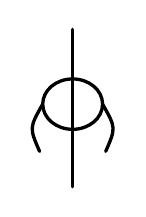
\begin{tikzpicture}[line width=1.2pt, line cap=round, line join=round]
  % Pole (vertical shaft)
  \draw (0,-0.9) -- (0,1.1);
  % Ring / target (slightly irregular, as in oracle bone style)
  \draw (0,0.15) ellipse (0.38 and 0.32);
  % Banner streamers (left and right, fluttering)
  \draw (-0.38,0.15) .. controls (-0.55,-0.15) .. (-0.42,-0.45);
  \draw ( 0.38,0.15) .. controls ( 0.55,-0.15) .. ( 0.42,-0.45);
\end{tikzpicture}

\smallskip
{\small\itshape zhǒng\,\raisebox{0.5ex}{\tiny$\checkmark$}}
\end{center}
